\documentclass{article}
\usepackage{amsmath}
\usepackage{graphicx}
\usepackage{hyperref} % Do klikalnych odnośników i referencji
\usepackage[utf8]{inputenc} % Obsługa polskich znaków
\usepackage[T1]{fontenc} % Poprawne kodowanie czcionek

\title{WSI - Lista 1}
\author{Tomasz Niedziałek}
\date{\today}

\begin{document}

\maketitle

\section{Wstęp} \label{sec:introduction}
Niniejsze sprawozdanie przedstawia wyniki trenowania sieci neuronowej do rozpoznawania cyfr z zestawu danych MNIST przy użyciu bibliotek TensorFlow i Keras. Wydajność sieci została oceniona na podstawie dokładności, precyzji i czułości na zbiorze testowym.

\section{Architektura modelu} \label{sec:model_architecture}
Model sieci neuronowej użyty w tym zadaniu to prosta sieć neuronowa typu feedforward o następującej architekturze:
\begin{itemize}
    \item Warstwa wejściowa: Kształt (28, 28)
    \item Warstwa spłaszczająca: Konwertuje dane wejściowe 2D na wektor 1D
    \item Warstwa gęsta: 128 jednostek z funkcją aktywacji ReLU
    \item Warstwa dropout: Współczynnik dropout 20\%
    \item Warstwa gęsta: 10 jednostek (warstwa wyjściowa)
\end{itemize}
Sieć neuronowa typu feedforward to najprostszy rodzaj sieci neuronowej, w której dane przepływają w jednym kierunku – od warstwy wejściowej, przez warstwy ukryte, aż do warstwy wyjściowej.

Funkcja aktywacji ReLU (Rectified Linear Unit) jest jedną z najczęściej używanych funkcji aktywacji w sieciach neuronowych. Zwraca wartość wejściową, jeśli jest dodatnia, lub 0, jeśli jest ujemna.

Dropout to technika regularizacji, która losowo "wyłącza" (zeruje) określony procent neuronów podczas treningu. W tym przypadku współczynnik dropout wynosi 20\%, co oznacza, że 20\% neuronów jest losowo wyłączanych w każdej iteracji. Technika ta pomaga zapobiegać przeuczeniu modelu (overfitting), zmuszając sieć do bardziej niezależnego uczenia się cech.

\section{Trenowanie i ewaluacja} \label{sec:training_evaluation}
Model był trenowany przez 10 epok z użyciem optymalizatora Adam i funkcji straty sparse categorical cross-entropy. Podczas procesu trenowania monitorowano dokładność i stratę na zbiorach treningowym i walidacyjnym.

Optymalizator Adam (Adaptive Moment Estimation) jest jedną z najczęściej używanych metod optymalizacji w uczeniu maszynowym. Adam dynamicznie dostosowuje współczynniki uczenia dla każdego parametru modelu, wykorzystując średnie ruchome gradientów (pierwszy moment) oraz ich kwadratów (drugi moment). Dzięki temu optymalizator Adam jest szybki, efektywny i dobrze sprawdza się w przypadku dużych zbiorów danych oraz modeli z dużą liczbą parametrów.

Funkcja straty sparse categorical cross-entropy jest używana w zadaniach klasyfikacji wieloklasowej, gdzie etykiety są reprezentowane jako liczby całkowite (np. 0, 1, 2, ...). Funkcja ta oblicza różnicę między przewidywanymi prawdopodobieństwami (wyjściem modelu) a rzeczywistymi etykietami klas. Minimalizacja tej funkcji pozwala modelowi poprawić swoje przewidywania, dostosowując wagi w sieci neuronowej.
\section{Wyniki} \label{sec:results}
Poniżej przedstawiono wyniki uzyskane podczas trenowania i ewaluacji modelu:

\begin{itemize}
    \item Początkowe wyjście softmax:
    \begin{verbatim}
    [[0.10025889, 0.10002384, 0.0999672, 0.09991807, 0.10014182, 
      0.10012015, 0.09991807, 0.09995951, 0.09994359, 0.09974883]]
    \end{verbatim}
    Wyjście softmax to wektor prawdopodobieństw, który reprezentuje przewidywania modelu dla każdej z 10 klas (cyfr od 0 do 9). Każda wartość w wektorze wskazuje prawdopodobieństwo, że dana próbka należy do danej klasy. Suma wszystkich wartości w wektorze wynosi 1.
    \item Początkowa strata: 2.3013842
    \item Końcowa dokładność treningowa: 91.51\%
    \item Końcowa dokładność walidacyjna: 87.03\%
    \item Końcowa dokładność testowa: 92.69\%
    \item Końcowa strata testowa: 0.2501
\end{itemize}
\section{Czułość i precyzja} \label{sec:precision_recall}
Poniżej przedstawiono wyniki dotyczące czułości, precyzji oraz miary F1 dla poszczególnych klas:

\begin{table}[h!]
\centering
\begin{tabular}{|c|c|c|c|c|}
\hline
\textbf{Klasa} & \textbf{Precyzja} & \textbf{Czułość} & \textbf{Miara F1} & \textbf{Liczność (support)} \\ \hline
0 & 0.94 & 0.98 & 0.96 & 980 \\ \hline
1 & 0.96 & 0.98 & 0.97 & 1135 \\ \hline
2 & 0.94 & 0.89 & 0.92 & 1032 \\ \hline
3 & 0.91 & 0.91 & 0.91 & 1010 \\ \hline
4 & 0.92 & 0.95 & 0.93 & 982 \\ \hline
5 & 0.90 & 0.88 & 0.89 & 892 \\ \hline
6 & 0.94 & 0.95 & 0.94 & 958 \\ \hline
7 & 0.93 & 0.94 & 0.93 & 1028 \\ \hline
8 & 0.88 & 0.89 & 0.89 & 974 \\ \hline
9 & 0.94 & 0.90 & 0.92 & 1009 \\ \hline
\textbf{Dokładność} & \multicolumn{4}{c|}{0.93 (na zbiorze testowym: 10000)} \\ \hline
\end{tabular}
\caption{Wyniki precyzji, czułości i miary F1 dla poszczególnych klas.}
\label{tab:precision_recall}
\end{table}

Poniżej przedstawiono macierz pomyłek (confusion matrix) dla modelu:

\begin{figure}[h!]
\centering
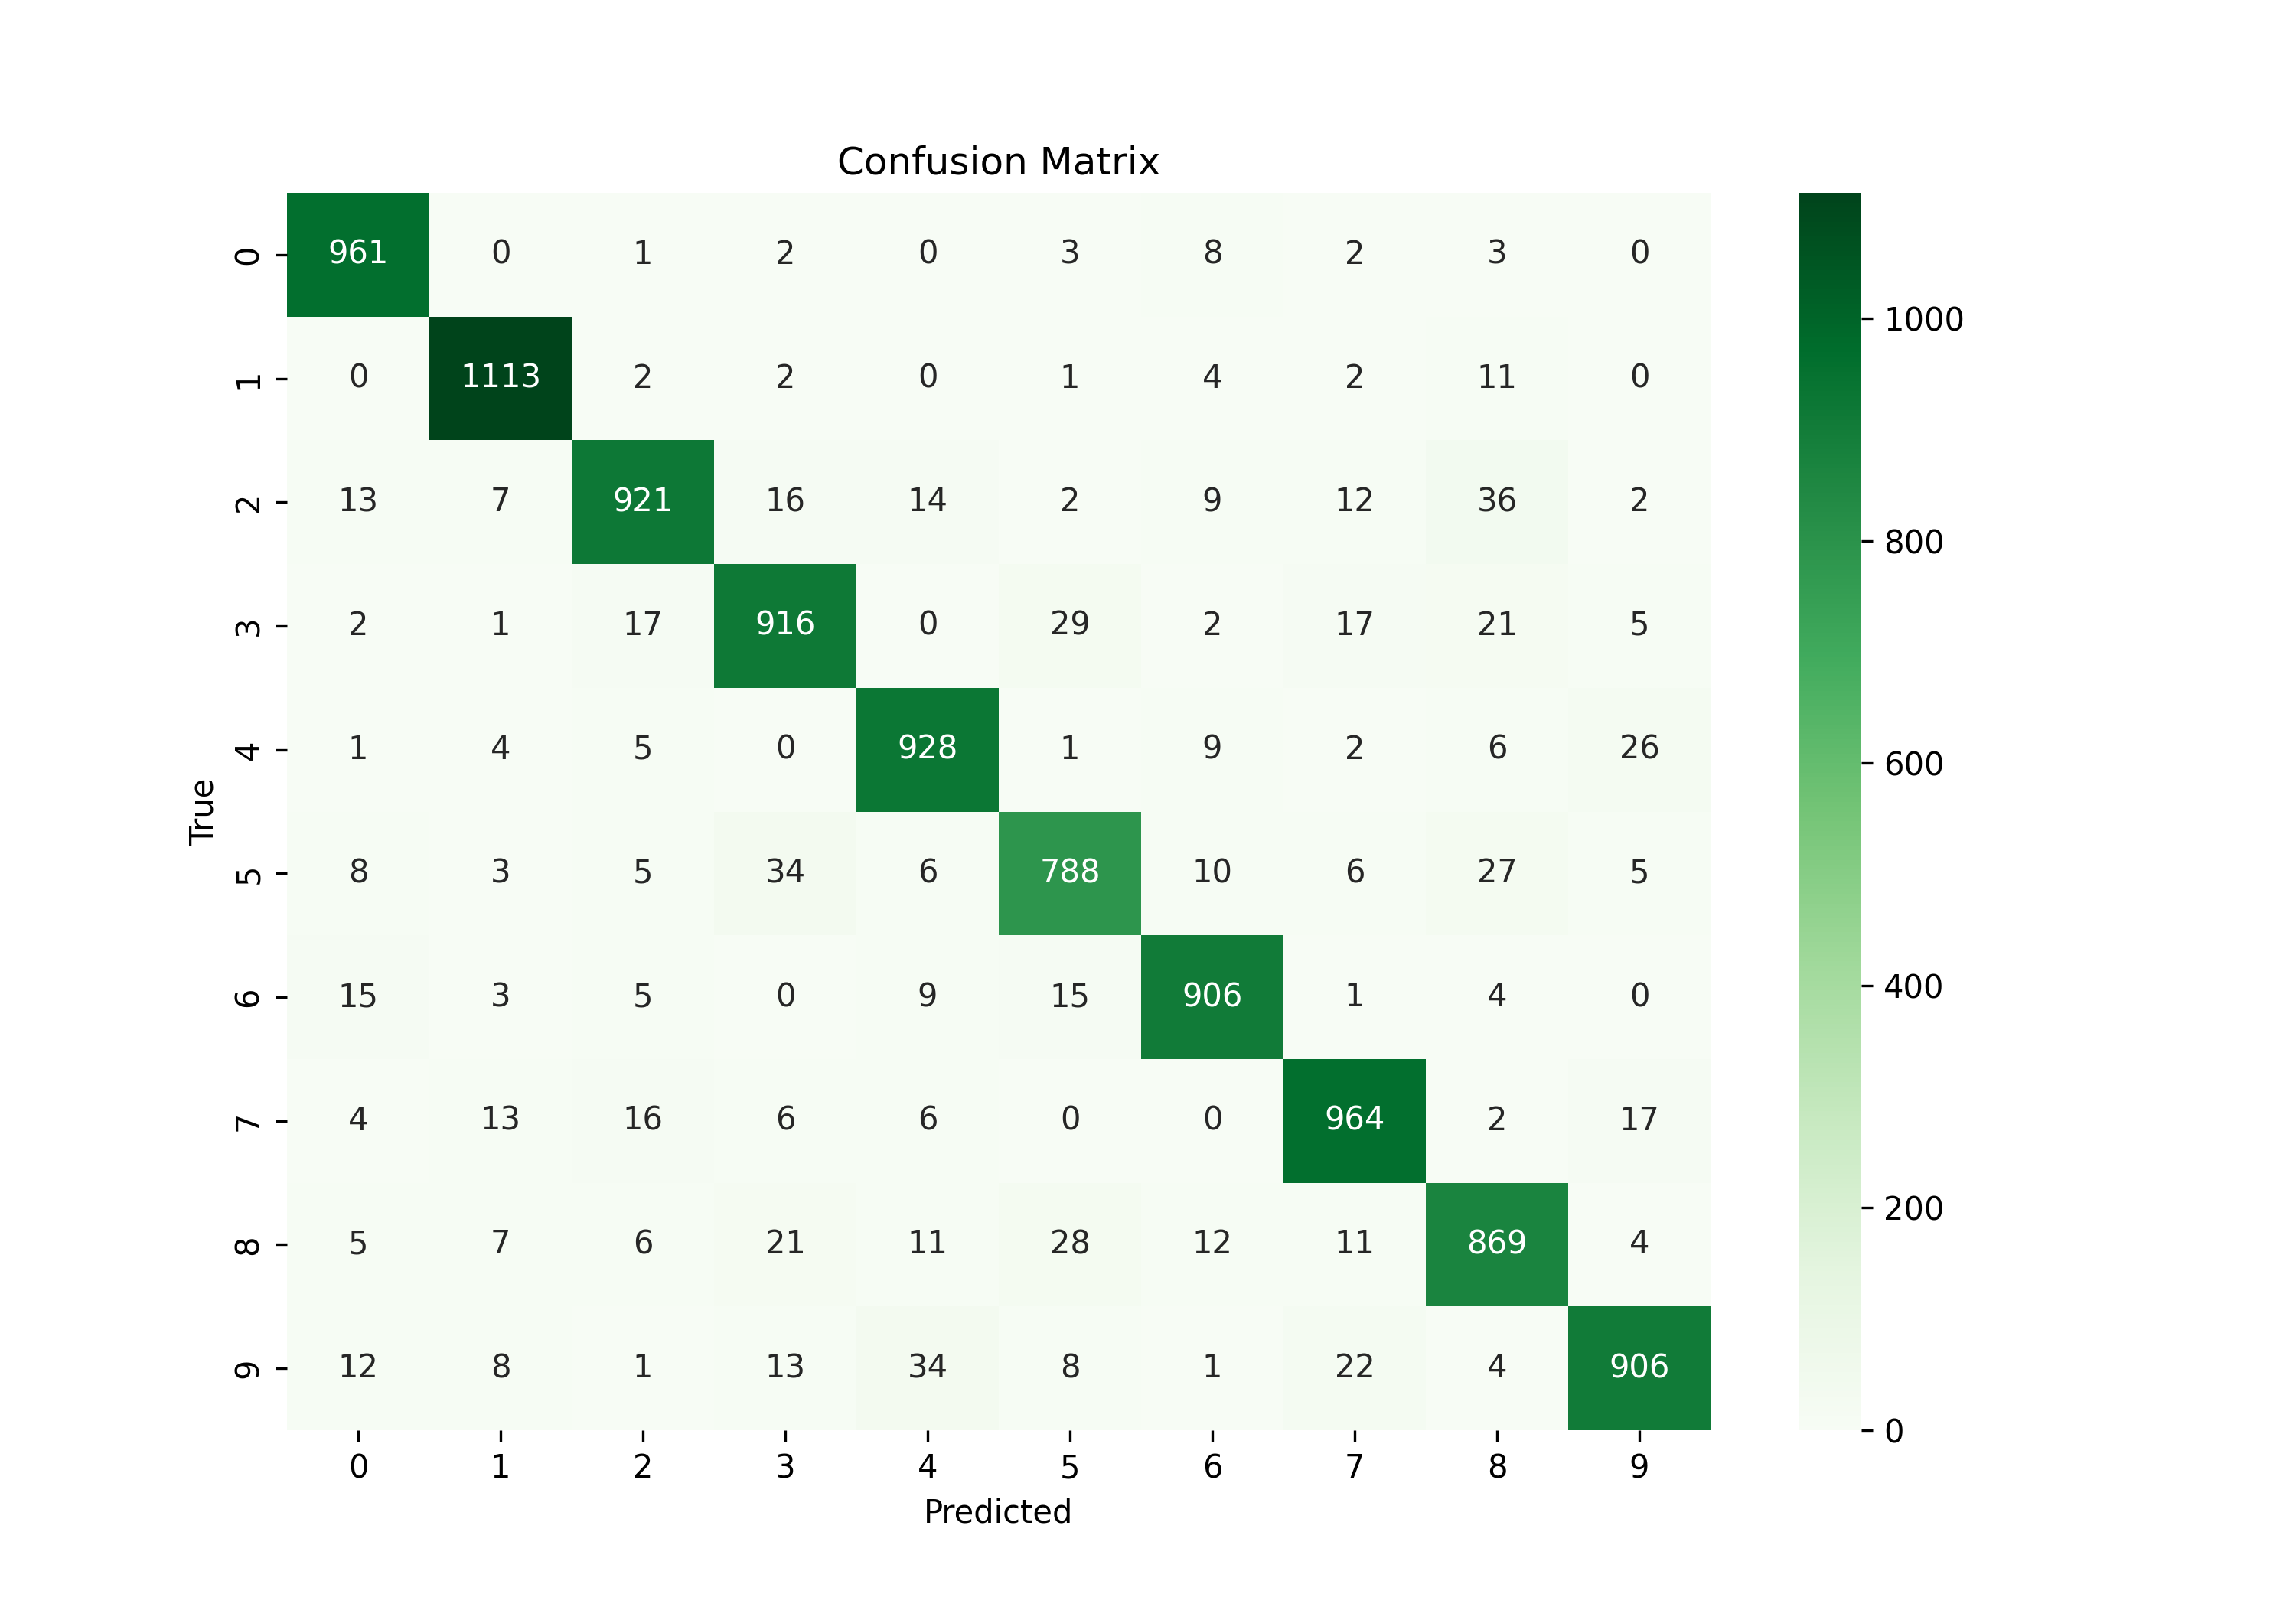
\includegraphics[width=0.8\textwidth]{confusion_matrix.png} 
\caption{Macierz pomyłek dla modelu.}
\label{fig:confusion_matrix}
\end{figure}

\section{Wnioski} \label{sec:conclusion}
Sieć neuronowa osiągnęła dokładność testową na poziomie 92.69\%, co wskazuje na dobrą wydajność w rozpoznawaniu cyfr z zestawu danych MNIST. Wysoka dokładność sugeruje, że model dobrze generalizuje na nieznane dane.

\section{Testowanie na własnych próbkach pisma}

\subsection{Wyniki testów}

Na podstawie własnych próbek pisma, stworzono zbiór testowy zawierający pięć egzemplarzy każdej cyfry. Sieć neuronowa, stworzona w poprzednim punkcie, została przetestowana na tym zbiorze. Poniżej przedstawiono wyniki testów:

\begin{itemize}
    \item Współczynnik rozpoznawalności: \textbf{34.00\%}
    \item Macierz pomyłek (confusion matrix): \\
    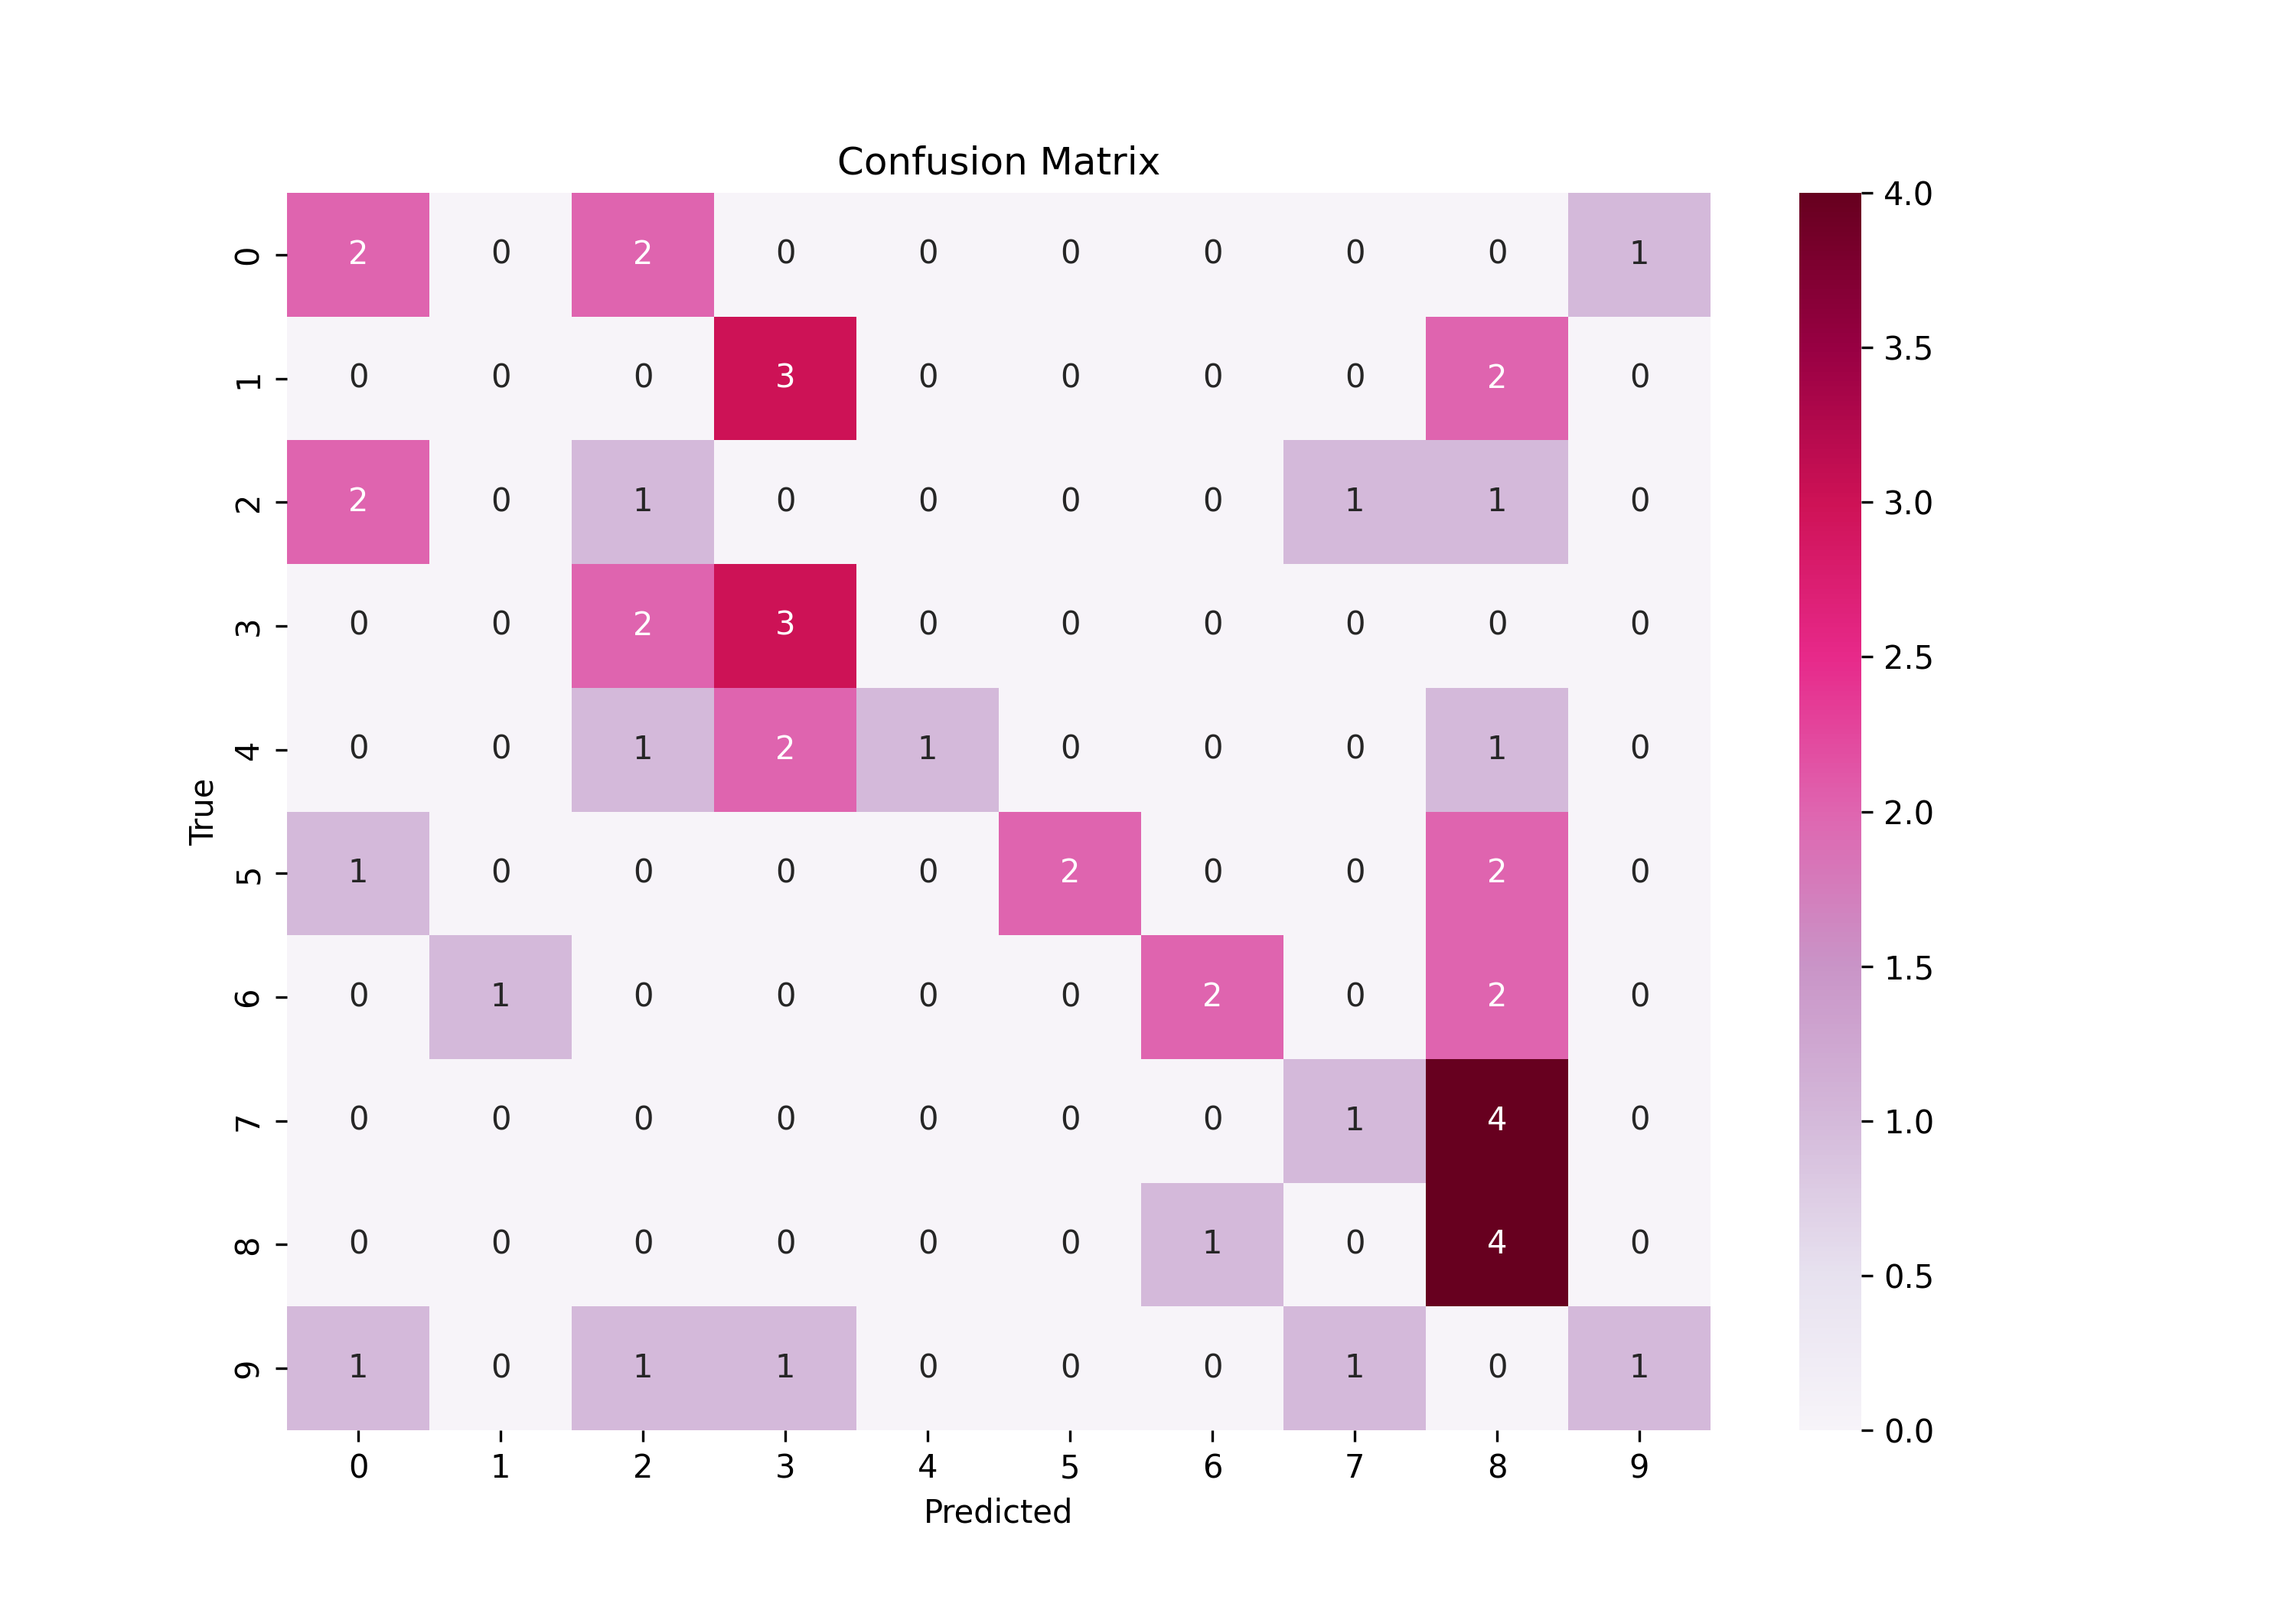
\includegraphics[width=0.8\textwidth]{confusion_matrix_my_digits.png}
\end{itemize}

\subsection{Wnioski}

Współczynnik rozpoznawalności na własnych próbkach pisma wyniósł \textbf{34.00\%}. Wynik ten jest znacznie niższy w porównaniu do wyników uzyskanych na zbiorze testowym MNIST, co może być spowodowane kilkoma czynnikami:

\begin{itemize}
    \item \textbf{Różnice w stylu pisma}: Własne próbki pisma mogą różnić się stylem od próbek w zbiorze MNIST, co utrudnia sieci neuronowej poprawne rozpoznanie cyfr.
    \item \textbf{Jakość próbek}: Jakość własnych próbek pisma może być niższa (np. rozmazane, nierówne linie), co wpływa na dokładność rozpoznawania.
    \item \textbf{Liczba próbek}: Mniejsza liczba próbek w zbiorze testowym może prowadzić do mniej reprezentatywnych wyników.
\end{itemize}

\subsection{Podsumowanie}

Testowanie sieci neuronowej na własnych próbkach pisma wykazało, że model ma trudności z rozpoznawaniem cyfr w różnych stylach pisma. Współczynnik rozpoznawalności wyniósł \textbf{34.00\%}. Aby poprawić wyniki, można rozważyć dalsze trenowanie modelu na większej liczbie próbek pisma, w tym na próbkach o różnych stylach i jakościach. Można również zastosować techniki augmentacji danych, aby zwiększyć różnorodność zbioru treningowego.

\section{Klasyfikator Random Forest do rozpoznawania cyfr} \label{sec:random_forest}

\subsection{Wyniki testów}

Klasyfikator Random Forest został wytrenowany i przetestowany na podanym zbiorze danych. Poniżej przedstawiono wyniki testów:

\begin{itemize}
    \item Współczynnik prawidłowej rozpoznawalności (Accuracy): \textbf{96.80\%}
    \item Precyzja, czułość oraz miara F1:
\end{itemize}

\begin{table}[h!]
\centering
\begin{tabular}{|c|c|c|c|c|}
\hline
Cyfra & Precyzja & Czułość & Miara F1 & Liczność (support) \\ \hline
0 & 0.97 & 0.99 & 0.98 & 980 \\ \hline
1 & 0.99 & 0.99 & 0.99 & 1135 \\ \hline
2 & 0.96 & 0.97 & 0.96 & 1032 \\ \hline
3 & 0.96 & 0.96 & 0.96 & 1010 \\ \hline
4 & 0.97 & 0.97 & 0.97 & 982 \\ \hline
5 & 0.97 & 0.97 & 0.97 & 892 \\ \hline
6 & 0.97 & 0.98 & 0.98 & 958 \\ \hline
7 & 0.97 & 0.96 & 0.96 & 1028 \\ \hline
8 & 0.96 & 0.95 & 0.96 & 974 \\ \hline
9 & 0.95 & 0.95 & 0.95 & 1009 \\ \hline
\end{tabular}
\caption{Wyniki precyzji, czułości i miary F1 dla poszczególnych cyfr w klasyfikatorze Random Forest.}
\label{tab:random_forest_metrics}
\end{table}

Poniżej przedstawiono macierz pomyłek (confusion matrix) dla klasyfikatora Random Forest:

\begin{figure}[h!]
\centering
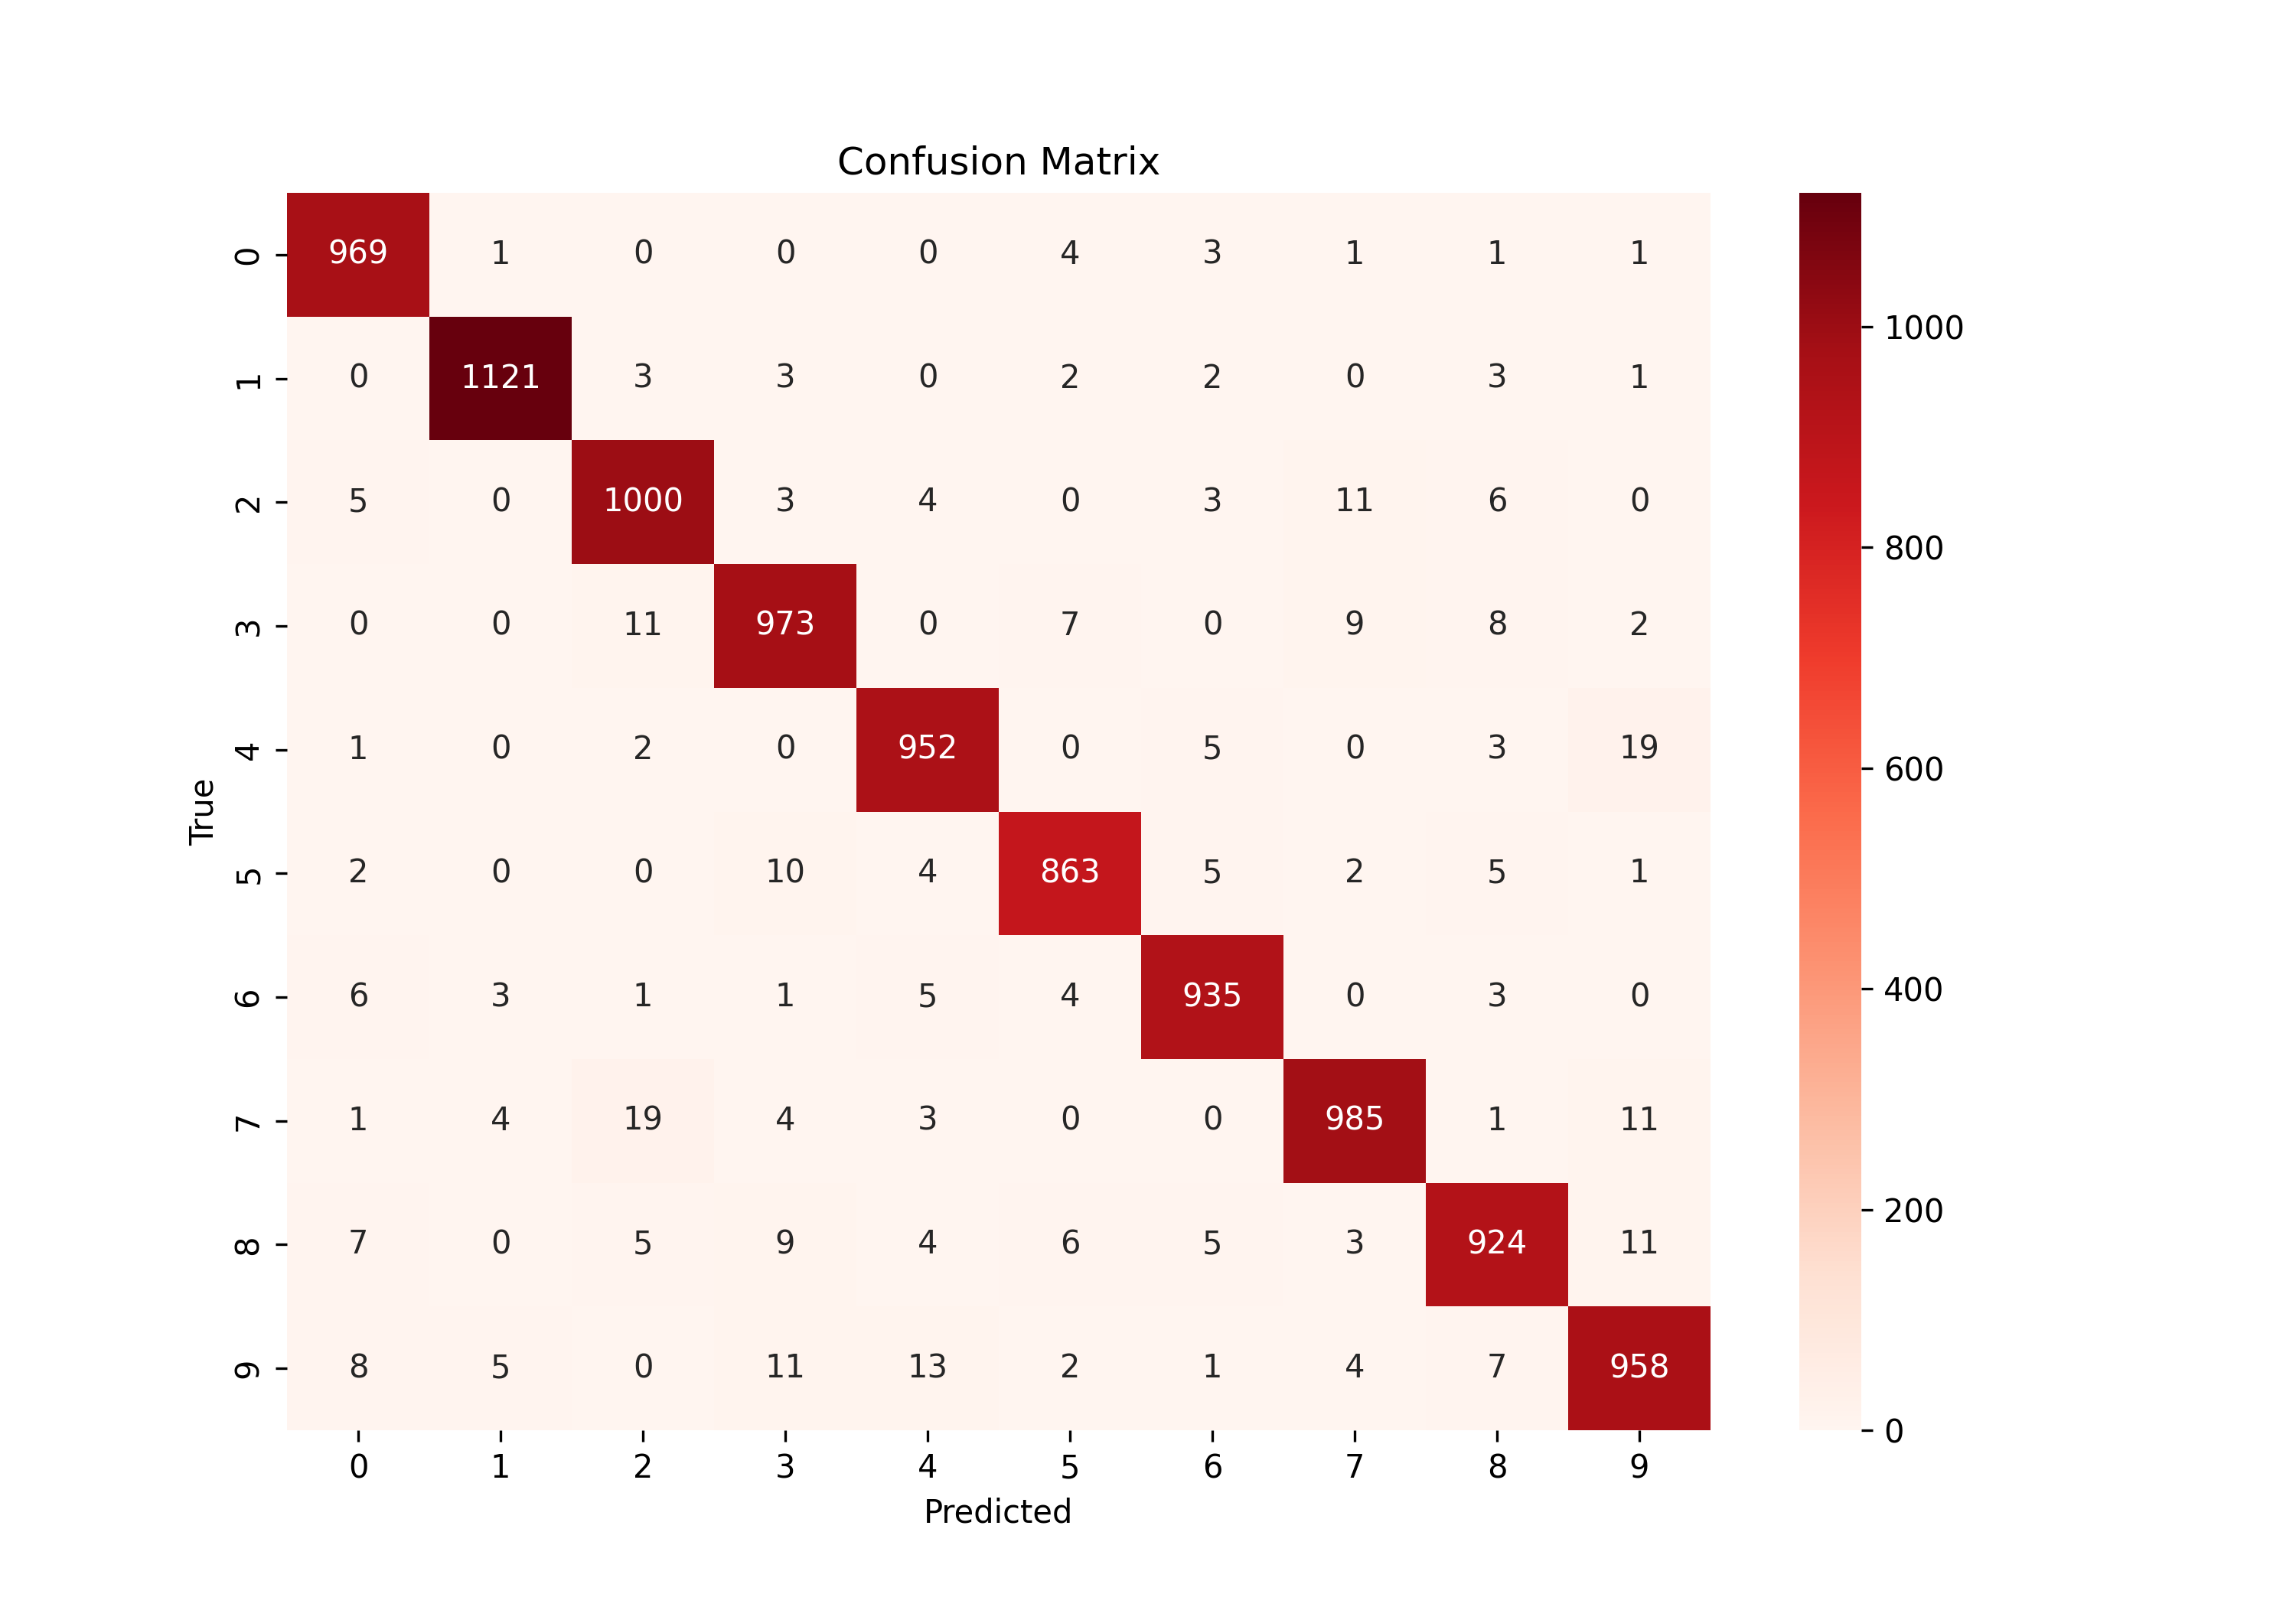
\includegraphics[width=0.8\textwidth]{confusion_matrix_random_forest.png} 
\caption{Macierz pomyłek dla klasyfikatora Random Forest.}
\label{fig:confusion_matrix_random_forest}
\end{figure}

\subsection{Wnioski}

Klasyfikator Random Forest osiągnął współczynnik prawidłowej rozpoznawalności na poziomie \textbf{96.80\%} na zbiorze testowym. Precyzja, czułość oraz miara F1 dla każdej cyfry zostały przedstawione w tabeli powyżej. Wysoka dokładność oraz zrównoważone wartości precyzji i czułości wskazują, że klasyfikator dobrze radzi sobie z rozpoznawaniem cyfr z podanego zbioru danych.
\end{document}